%&pdflatex
\documentclass[
aps,%
12pt,%
final,%
notitlepage,%
oneside,%
onecolumn,%
nobibnotes,%
nofootinbib,%
superscriptaddress,%
noshowpacs,%
showkeys,%
floatfix,% for ContinuedFloat figures
tightenlines,%
centertags]%
{revtex4}

\usepackage{wrapfig}
\usepackage{mathrsfs}   % for mathscr
\usepackage{mathtools}  % for multlined

%%% breaking long formulas
\allowdisplaybreaks[3]

\usepackage[caption=false]{subfig}
\renewcommand{\thesubfigure}{\asbuk{subfigure}}

\PassOptionsToPackage{monochrome}{xcolor}
\usepackage{tikz}
\usepackage{pgfplots}

\newcommand{\Kn}{\mathrm{Kn}}
\newcommand{\Ma}{\mathrm{Ma}}
\newcommand{\Sh}{\mathrm{Sh}}
\newcommand{\dd}{\mathrm{d}}
\newcommand{\pder}[2][]{\frac{\partial#1}{\partial#2}}
\newcommand{\pderdual}[2][]{\frac{\partial^2#1}{\partial#2^2}}
\newcommand{\pderder}[3][]{\frac{\partial^2#1}{\partial#2\partial#3}}
\newcommand{\Pder}[2][]{\partial#1/\partial#2}
\newcommand{\Pderdual}[2][]{\partial^2#1/\partial#2^2}
\newcommand{\Pderder}[3][]{\partial^2#1/\partial#2\partial#3}
\newcommand{\dzeta}{\boldsymbol{\dd\zeta}}
\newcommand{\dxi}{\boldsymbol{\dd\xi}}
\newcommand{\bzeta}{\boldsymbol{\zeta}}
\newcommand{\deltann}[2]{(\delta_{#1#2}-n_#1 n_#2)}
\newcommand{\bxi}{\boldsymbol{\xi}}
\newcommand{\bh}{\boldsymbol{h}}
\newcommand{\be}{\boldsymbol{e}}
\newcommand{\Nu}{\mathcal{N}}
\newcommand{\Mu}{\mathcal{M}}
\newcommand{\OO}[1]{O(#1)}
\newcommand{\oo}[1]{o(#1)}
\newcommand{\onwall}[1]{\left(#1\right)_0}
\newcommand{\Set}[2]{\{\,{#1}:{#2}\,\}}

\begin{document}
\selectlanguage{russian}

\title{Медленные неизотермические течения: численный и асимптотический анализ уравнения Больцмана}
\author{\firstname{О.~А.}~\surname{Рогозин}}
\email{oleg.rogozin@phystech.edu}
\affiliation{Moсковский физико-технический институт}

\date{\today}

\begin{abstract}
    \begin{flushright}
    \vspace{1em}
    {\it Памяти Оск\'{а}ра Гаврииловича Фридлендера (1939--2015)}
    \vspace{1em}
    \end{flushright}
    Рассматриваются медленные течения слаборазреженного газа
    под действием значительных температурных напряжений.
    Для корректного гидродинамического описания этого класса течений
    используются уравнения Когана"--~Галкина"--~Фридлендера,
    содержащие в уравнении импульса некоторые ненавье"--~стокстовские члены.
    Соответствующие граничные условия определяются из
    асимтотического анализа кнудсеновского слоя на основе уравнения Больцмана.
    Изучается вопрос постановки граничных условий вплоть до второго порядка малости по числу Кнудсена.
    На нескольких примерах проводится их сравнительный анализ.
    Результаты подкрепляются численным решением уравнения Больцмана на основе
    проекционно-интерполяционного метода дискретных скоростей для неравномерных сеток.
    Впервые получена картина конкуренции нелинейной термострессовой конвекции с
    нелинейными течениями следующего порядка малости по числу Кнудсена.
\end{abstract}

\keywords{
    уравнение Больцмана,
    уравнения Когана"--~Галкина"--~Фридлендера,
    нелинейное термострессовое течение,
    проекционный метод,
    OpenFOAM
}

\maketitle

%%%%%%%%%%%%%%%%%%%%%%%%%%%%%%%%%%%%%%%%%%%
\section{Введение}
%%%%%%%%%%%%%%%%%%%%%%%%%%%%%%%%%%%%%%%%%%%

%%% Slow nonisothermal flows
С 1969 по 1974 год Оск\'{а}р Гавриилович Фридлендер (1939--2015)
совместно с Владленом Сергеевичем Галкиным (род.~1932)
под руководством Михаила Наумовича Когана (1925--2011)
развили теорию \emph{медленных неизотермических}
течений газа~\cite{Kogan1970, Kogan1971, Friedlander1974, Galkin1974, Kogan1976}.
Медленность течений следует понимать как малость числа Маха (\(\Ma\ll1\)),
а неизотермичность как присутствие в газе существенного градиента температур.
Основным импульсом упомянутых работ стала попытка учесть влияние температурных напряжений
на конвекцию газа через анализ барнеттовского приближения слаборазреженного газа.
Несмотря на то что барнеттовские члены второго порядка малости по числу Кнудсена \(\Kn\),
при \(\Ma\sim\Kn\) (число Рейнольдса порядка единицы)
они становятся сравнимыми с ньютоновскими вязкостными напряжениями.
Таким образом, уравнения Навье"--~Стокса оказываются некорректными для
описания медленных неизотермических течений.

%%% KGF equations and its derivation
В~\cite{Kogan1970} впервые была получена система уравнений гидродинамического типа,
корректно описывающая медленные неизотермические течения слаборазреженного газа.
В литературе нет единого устоявшегося их названия,
поэтому автор предлагает ввести термин \emph{уравнения Когана"--~Галкина"--~Фридлендера}
или \emph{уравнения КГФ}.
В первых работах~\cite{Kogan1970, Kogan1971} эти уравнения были получены наиболее простым способом,
на основе разложения Чепмена"--~Энскога. Такие же уравнения получаются из разложения Гильберта~\cite{Galkin1974}.
Наиболее общая формулировка нестационарных уравнений КГФ для смеси газов изложена в~\cite{Galkin2015}.

%%% Transport coefficients
Кроме коэффициентов вязкости и теплопроводности, в уравнения КГФ входят некоторые
\emph{термострессовые} транспортные коэффициенты. Для некоторых молекулярных потенциалов они
были впервые вычислены с помощью полиномов Сонина~\cite{Burnett1935, Chapman1960}.
Для газа твёрдых сфер более точные значения получены с помощью
непосредственного численного решения соответствующих интегральных уравнений~\cite{Sone1996, Sone2002, Sone2007}.

%%% Nonlinear thermal-stress flow and its simulation
Нелинейный характер температурных напряжений в уравнениях КГФ приводит к
явлению конвекции газа под их действием (\emph{нелинейная термострессовая} конвекция)~\cite{Kogan1971}.
Этот тип конвекции имеет место при отсутствии внешних сил и может возникать между равномерно нагретыми телами.
Нелинейные температурные напряжения при некоторых условиях влияют также на процессы теплопередачи~\cite{Friedlander1978}.
В результате многолетнего труда под руководством О.\,Г. Фридлендера теория медленных неизотермических течений
была подтверждена экспериментально~\cite{Friedlander1997, Friedlander2003}.
В это же время, благодаря развитию вычислительной техники, появилась возможность провести численный анализ
некоторых прикладных задач с помощью уравнений КГФ, а также кинетических уравнений:
на основе модельных уравнений~\cite{Alexandrov2002, Aoki2006, Alexandrov2008b, Alexandrov2011, Rykov2008}
и прямого статистического моделирования (DSMC)~\cite{Alexandrov2008a, Aoki2007}.

%%% Requirements to the numerical methods
Для малых чисел Кнудсена и особенно медленных течений, стохастические методы крайне трудоёмки с вычислительной точки зрения,
а получаемые с их помощью решения страдают от высокого уровня статистического шума.
Детерминистические методы решения уравнения Больцмана весьма перспективны в этой области~\cite{Dimarco2014,Mieussens2014},
однако связанные с ними вычислительные трудности не были преодолены полностью до настоящего времени.
По этой причине какие-либо результаты моделирования нелинейных термострессовых течений
на основе уравнения Больцмана, требующие от численного метода высокой точности, в литературе не представлены.
Кроме того, эти течения не могут наблюдаться в одномерных задачах.
Существенную сложность представляет высокоточный анализ приграничной области~\cite{Takata2015second},
особенно около выпуклых поверхностей~\cite{Takata2015curvature},
где функция распределения испытывает значительные перепады.
Медленные течения с большим перепадом температур предъявляют дополнительные требования к сетке в скоростном пространстве.
Она должна удовлетворительно аппроксимировать функцию распределения как холодного газа,
так и горячего, что требует измельчения сетки для малых молекулярных скоростей наравне с её большим объёмом.
Обобщение проекционно-интерполяционного метода~\cite{Tcheremissine1997, Tcheremissine2000}
на неравномерные сетки~\cite{Rogozin2016} на основе методики многоточечного проецирования~\cite{Dodulad2012}
позволяет эффективно решать рассматриваемый класс задач.

%%% Continuum limit
Асимптотический анализ уравнения Больцмана для медленных неизотермических течений
показывает, что стационарное уравнение теплопроводности некорректно описывает
разреженный газ в континуальном пределе (\(\Kn\to0\))~\cite{Bobylev1995}.
Этот факт подтверждается также численным анализом~\cite{Sone1996}.
Оказывается, что инфинитезимальное поле скоростей конечным образом влияет на температурное поле.
Такое асимптотическое поведение было названо \emph{призрак-эффектом} (ghost effect)~\cite{Sone2002, Sone2007}.
Некоторые математические вопросы существования и устойчивости решений уравнений КГФ
обсуждаются в~\cite{Levermore2012, Levermore2015, Tan2016}.

%%% Boundary conditions
До настоящего времени уравнения КГФ решались численно только
с граничными условиями теплового скольжения (thermal creep).
Это естественные условия для уравнений ведущего порядка,
однако решение может быть улучшено, если учесть некоторые граничные условия следующего порядка,
например температурного и скоростного скачков, термострессового скольжения (thermal-stress slip),
а также влияние кривизны граничной поверхности.
Это оказывается возможным, поскольку для постановки этих условий достаточно
знания гидродинамического решения ведущего порядка и некоторых его производных.

%%%%%%%%%%%%%%%%%%%%%%%%%%%%%%%%%%%%%%%%%%%
\section{Основные уравнения}
%%%%%%%%%%%%%%%%%%%%%%%%%%%%%%%%%%%%%%%%%%%

Прежде всего, перейдём к безразмерным переменным.
Пусть \(L\) "--- характерная длина в рассматриваемой задаче,
а \(T^{(0)}\) и \(p^{(0)}\) "--- характерные температура и давление газа.
Тогда макроскопические переменные принимают следующий вид:
температура \(TT^{(0)}\), давление \(pp^{(0)}\),
плотность \(\rho p^{(0)}/RT^{(0)}\), скорость \(v_i(2RT^{(0)})^{1/2}\).
Функция распределения молекулярных скоростей \(f(x_i,\zeta_i)(2p^{(0)})/(2RT^{(0)})^{5/2}\)
определяется в физическом пространстве \(x_iL\) и скоростном \(\zeta_i(2RT^{(0)})^{1/2}\).
Удельная газовая постоянная \(R = k_B/m\), где \(k_B\) "--- постоянная Больцмана,
\(m\) "--- масса молекулы.
Число Кнудсена \(\Kn = \ell^{(0)}/L\) определяется через характерную длину свободного пробега
\begin{equation}\label{eq:ell}
    \ell^{(0)} = \frac{k_B T^{(0)}}{\sqrt2\pi d_m^2 p^{(0)}},
\end{equation}
где радиус действия межмолекулярного потенциала взаимодействия \(d_m\)
совпадает с диаметром молекул для газа твёрдых сфер.

Стационарное уравнение Больцмана в присутствии внешней силы \(F_i (2RT^{(0)})/L\) в безразмерных переменных имеет вид:
\begin{equation}\label{eq:Boltzmann}
    \zeta_i\pder[f]{x_i} + F_i\pder[f]{\zeta_i} = \frac1k J(f,f),
\end{equation}
где интеграл столкновений
\begin{equation}\label{eq:integral}
    J(f,g) = \frac12 \int(f'g'_*+g'f'_*-fg_*-gf_*)B\dd\Omega(\boldsymbol\alpha) \dzeta_*
\end{equation}
и \(k = \sqrt\pi\Kn/2\).
\(\Omega(\boldsymbol{\alpha})\) "--- телесный угол в направлении единичного вектора \(\boldsymbol\alpha\),
\(B\) "--- функционал межмолекулярного потенциала. Для газа твёрдых сфер,
\begin{equation}\label{eq:ci_kernel}
    B = \frac{|\alpha_i(\zeta_{i*}-\zeta_i)|}{4\sqrt{2\pi}}.
\end{equation}
Макроскопические переменные выражаются через моменты функции распределения:
\begin{equation}\label{eq:macro}
    \rho = \int f \dzeta, \quad
    v_i = \frac1{\rho} \int \zeta_i f \dzeta, \quad
    T = \frac{2}{3\rho}\int(\zeta_i-v_i)^2 f \dzeta, \quad
    p = \rho T.
\end{equation}

Граничные условия диффузного отражения задаются следующим образом:
\begin{equation}\label{eq:diffuse_bc}
    f\left(\zeta_i n_i > 0\right) =
        \frac{\sigma_B}{(\pi T_B)^{3/2}} \exp\left(-\frac{\zeta_i^2}{T_B}\right), \quad
    \sigma_B = -2\left(\frac{\pi}{T_B}\right)^{1/2} \int_{\zeta_i n_i < 0} \zeta_j n_j f\dzeta,
\end{equation}
где \(n_i\) "--- единичный вектор нормали к границе, направленный внутрь газа,
а \(T_B\) и \(v_{Bi}\) "--- граничные температура и скорость.
Для стационарных задач предполагается, что \(v_{Bi}n_i = 0\).

%%%%%%%%%%%%%%%%%%%%%%%%%%%%%%%%%%%%%%%%%%%
\section{Асимптотический анализ}
%%%%%%%%%%%%%%%%%%%%%%%%%%%%%%%%%%%%%%%%%%%

В этом разделе кратко излагаются основные результаты асимптотической теории
медленных неизотермических течений на основе разложения Гильберта.
Используются обозначения, принятые в~\cite{Sone2002, Sone2007}.
Для простоты рассматривается только молекулярная модель упругих сфер.

При малых \(k\) решение стационарного уравнения Больцмана допускает разделение пространственных масштабов,
так что оно может быть найдено в форме
\begin{equation}\label{eq:sum_solutions}
    f = f_H + f_K,
\end{equation}
где \(f_H\) "--- гидродинамическая часть решения с масштабом порядка единицы,
\(f_K\) "--- коррекция кнудсеновского слоя с масштабом порядка \(k\).
Такое разделение возможно, поскольку \(f_K\) убывает экспоненциально по мере удаления от границы.
Нелинейная теория возмущений позволяет отыскать \(f_H\),
зависящее только от макроскопических переменных и их производных,
однако полученное решение не обладает достаточным количеством степеней свободы,
чтобы удовлетворить граничному условию диффузного отражения~\eqref{eq:diffuse_bc}.
Численное решение задачи кнудсеновского слоя позволяет найти \(f_K\),
а также граничные условия для \(f_H\).

\subsection{Гидродинамическая часть решения}

Функция распределения \(f_H\) и макроскопические переменные \(h_H = \rho_H, v_{iH}, T_H, \dots\)
могут быть разложены в ряд по \(k\):
\begin{equation}\label{eq:expansion}
    f_H = f_{H0} + f_{H1}k + f_{H2}k^2 + \cdots, \quad h_H = h_{H0} + h_{H1}k + h_{H2}k^2 + \cdots.
\end{equation}
Будем искать решение уравнения Больцмана в предположении,
что \(\Pder[f_H]{x_i} = \OO{f_H}\) (разложение Гильберта),
\(v_{iH0} = 0\) (медленные течения), \(F_{iH0} = F_{iH1} = 0\) (слабое поле внешних сил).
Подставляя~\eqref{eq:expansion} в уравнение Больцмана~\eqref{eq:Boltzmann} и приравнивая члены
при равных степенях \(k\), получаем систему интегро-дифференциальных уравнений,
для которой должны выполняться условия разрешимости. В нулевом порядке
\begin{equation}
    \pder[p_{H0}]{x_i} = 0. \label{eq:asymptotic0_p}
\end{equation}
В первом
\begin{gather}
    \pder{x_i}\left(\frac{u_{iH1}}{T_{H0}}\right) = 0, \label{eq:asymptotic1_u} \\
    \pder[p_{H1}]{x_i} = 0, \label{eq:asymptotic1_p} \\
    \pder[u_{iH1}]{x_i} = \frac{\gamma_2}2\pder{x_i}\left(\sqrt{T_{H0}}\pder[T_{H0}]{x_i}\right). \label{eq:asymptotic1_T}
\end{gather}
Во втором при \(p_{H1} = 0\)
\begin{gather}
    \pder{x_i}\left(\frac{u_{iH2}}{T_{H0}}\right)
        = \frac{u_{iH1}}{T_{H0}}\pder{x_i}\left(\frac{T_{H1}}{T_{H0}}\right), \label{eq:asymptotic2_u} \\
    \begin{aligned}
        \pder{x_j}\left(\frac{u_{iH1}u_{jH1}}{T_{H0}}\right)
        &-\frac{\gamma_1}2\pder{x_j}\left[\sqrt{T_{H0}}\left(
            \pder[u_{iH1}]{x_j} + \pder[u_{jH1}]{x_i} - \frac23\pder[u_{kH1}]{x_k}\delta_{ij}
        \right)\right] \\
        &- \frac{\bar{\gamma}_7}{T_{H0}}\pder[T_{H0}]{x_i}\pder[T_{H0}]{x_j}\left(\frac{u_{jH1}}{\gamma_2\sqrt{T_{H0}}} - \frac{1}4\pder[T_{H0}]{x_j}\right)
        = -\frac12\pder[p_{H2}^\dag]{x_i} + \frac{p_{H0}^2 F_{iH2}}{T_{H0}},
    \end{aligned} \label{eq:asymptotic2_p} \\
    \pder[u_{iH2}]{x_i} = \frac{\gamma_2}2\pderdual{x_i}\left(T_{H1}\sqrt{T_{H0}}\right). \label{eq:asymptotic2_T}
\end{gather}
Здесь введены следущие обозначения: \(u_{iH1} = p_{H0}v_{iH1}\), \(u_{iH2} = p_{H0}v_{iH2}\) и
\begin{equation}\label{eq:dag_pressure}
    p_{H2}^\dag = p_{H0} p_{H2}
        + \frac{2\gamma_3}{3}\pder{x_k}\left(T_{H0}\pder[T_{H0}]{x_k}\right)
        - \frac{\bar{\gamma}_7}{6}\left(\pder[T_{H0}]{x_k}\right)^2.
\end{equation}
Уравнения~\eqref{eq:asymptotic1_u},~\eqref{eq:asymptotic1_T},~\eqref{eq:asymptotic2_p}
для \(T_{H0}\), \(u_{iH1}\) и \(p_{H2}^\dag\) будем называть \emph{уравнениями Когана"--~Галкина"--~Фридлендера}.
Они содержат член температурных напряжений, отсутствующий в уравнениях Навье"--~Стокса.
Сравнивая его с \(p_{H0}^2F_{iH2}/T_{H0}\), можно увидеть, что на единицу массы газа действует сила
\begin{equation}\label{eq:gamma7_force}
    k^2\frac{\bar{\gamma}_7}{p_{H0}^2}\pder[T_{H0}]{x_i}\pder[T_{H0}]{x_j}\left(\frac{u_{jH1}}{\gamma_2\sqrt{T_{H0}}} - \frac{1}4\pder[T_{H0}]{x_j}\right).
\end{equation}
Она возникает, когда изотермические поверхности не параллельны:
\begin{equation}\label{eq:nonparallel}
    e_{ijk}\pder[T_{H0}]{x_j}\pder{x_k}\left(\pder[T_{H0}]{x_l}\right)^2 \ne 0.
\end{equation}
В~\eqref{eq:nonparallel} использован символ Леви"--~Чивиты \(e_{ijk}\).
Движение газа под действием этой силы называется \emph{нелинейным термострессовым} течением~\cite{Sone2002,Sone2007}.

Важно отметить, что \(p_{H2}^\dag\) не входит непосредственно в уравнение состояния,
поэтому определяется с точностью до константы.
Поскольку член \(\partial{p_{H2}^\dag}/\partial{x_i}\) включён в систему,
как давление в уравнениях Навье"--~Стокса для несжимаемого газа,
то для решения уравнений КГФ применяются соответствующие численные методы.

Безразмерные транспортные коэффициенты для газа твёрдых сфер:
\begin{alignat*}{2}\label{eq:gamma_coeffs}
    \gamma_1 &= 1.270042427, &\quad \gamma_2 &= 1.922284066, \\
    \gamma_3 &= 1.947906335, &\quad \bar{\gamma}_7 &= 1.758705.
\end{alignat*}
Первые два из них соответствуют вязкости \(\mu\) и теплопроводности \(\lambda\) газа,
\begin{equation}\label{eq:mu_lambda}
    \mu = \gamma_1\sqrt{T_{H0}} \frac{p^{(0)}L}{\sqrt{2RT^{(0)}}} k, \quad
    \lambda = \frac{5\gamma_2}{2}\sqrt{T_{H0}} \frac{p^{(0)}RL}{\sqrt{2RT^{(0)}}} k.
\end{equation}
Коэффициент \(\gamma_3\) входит в выражения температурных напряжений,
которые создают неоднородное распределение давления в газе,
но не движущую силу. Поскольку \(\bar{\gamma}_7\) положителен,
нелинейная термострессовая конвекция противоположна градиенту температур.

\subsection{Слой Кнудсена и граничные условия}

Граничное условие диффузного отражения~\eqref{eq:diffuse_bc} может быть удовлетворено,
если предположить, что \(f_K\) убывает экспоненциально на расстоянии порядка длины свободного пробега:
\begin{gather}
    k n_i\pder[f_K]{x_i} = \OO{f_K}, \quad k\to0, \label{eq:knlayer_sharp}\\
    f_K = \oo{\eta^{-m}}, \quad \eta\to\infty, \quad m\in\mathbb{N}. \label{eq:knlayer_exp}
\end{gather}
Здесь использованы естественные для слоя Кнудсена переменные:
\begin{equation}\label{eq:eta_definition}
    x_i = k\eta n_i(\chi_1,\chi_2) + x_{Bi}(\chi_1,\chi_2),
\end{equation}
где \(x_{Bi}\) "--- граничная поверхность, \(\eta\) "--- координата, растянутая вдоль нормали \(n_i\),
\(\chi_1\) и \(\chi_2\) "--- ортогональные координаты поверхности \(\eta=const\).
Тогда \(f_K\) подчиняется уравнению
\begin{equation}\label{eq:fK_equation}
    \zeta_in_i\pder[f_K]{\eta} = 2J(f_H,f_K) + J(f_K,f_K)
    - k\zeta_i\left(\pder[\chi_1]{x_i}\pder[f_K]{\chi_1} + \pder[\chi_2]{x_i}\pder[f_K]{\chi_2}\right).
\end{equation}

В нулевом порядке гидродинамическая часть решения является максвеллианом
\begin{equation}\label{eq:fH0_solution}
    f_{H0} = \frac{\rho_{H0}}{(\pi T_{H0})^{3/2}}\exp\left(-\frac{\zeta_i^2}{T_{H0}}\right),
\end{equation}
который удовлетворяет граничному условию~\eqref{eq:diffuse_bc} при
\begin{equation}\label{eq:boundary_T0}
    T_{H0} = T_{B0},
\end{equation}
а значит \(f_{K0} = 0\). Используя разложения
\begin{gather}
    f_K = f_{K1}k + f_{K2}k^2 + \cdots, \label{eq:knlayer_expansion}\\
    f_H = \onwall{f_{H0}} + \left[\onwall{f_{H1}} + \eta\onwall{\pder[f_{H0}]{x_i}}n_i \right]k + \cdots, \label{eq:Honwall_expansion}
\end{gather}
где \(\onwall{\cdots}\) означает значение на границе (\(\eta=0\)),
получаем уравнения для \(f_{K1}\) и \(f_{K2}\):
\begin{gather}
    \zeta_in_i\pder[f_{K1}]{\eta} = 2J\left[\onwall{f_{H0}},f_{K1}\right], \label{eq:knlayer1}\\
    \begin{multlined}
        \zeta_in_i\pder[f_{K2}]{\eta} = 2J\left[\onwall{f_{H0}}, f_{K2}\right]
        - \zeta_i\left[\onwall{\pder[\chi_1]{x_i}}\pder[f_{K1}]{\chi_1} + \onwall{\pder[\chi_2]{x_i}}\pder[f_{K1}]{\chi_2}\right] \\
        + 2J\left[\onwall{f_{H1}}+\eta\onwall{\pder[f_{H0}]{x_i}}n_i,f_{K1}\right] + J(f_{K1},f_{K1}).
    \end{multlined}\label{eq:knlayer2}
\end{gather}
При соответствующих граничных условиях в полупространстве \(\eta>0\) существует единственное решение
одномерного линеаризованного (около максвеллиана \(f_{H0}\) на границе) уравнения Больцмана~\eqref{eq:knlayer1}
тогда и только тогда, когда граничные значения \(\tau_{H1}\) и \(u_{jH1}\deltann{i}{j}\)
принимают определённые значения~\cite{Maslova1982, Bardos1986}.
Аналогичное утверждение имеет место для уравнения~\eqref{eq:knlayer2}
и граничных значений \(\tau_{H2}\) и \(u_{jH2}\deltann{i}{j}\).

Однородное уравнение~\eqref{eq:knlayer1} приводит к следующим
граничным условиям и коррекциям кнудсеновского слоя:
\begin{gather}
    \frac1{\sqrt{T_{B0}}}\begin{bmatrix} (u_{jH1} - u_{Bj2}) \\ u_{jK1} \end{bmatrix} \deltann{i}{j} =
        - \onwall{\pder[T_{H0}]{x_j}} \deltann{i}{j}
        \begin{bmatrix} K_1 \\ \frac12 Y_1(\tilde\eta) \end{bmatrix}, \label{eq:boundary_u1t}\\
    \begin{bmatrix} u_{jH1} \\ u_{jK1} \end{bmatrix} n_j = 0, \label{eq:boundary_u1n}\\
    \frac{p_{H0}}{T_{B0}}\begin{bmatrix} T_{H1} - T_{B1} \\ T_{K1} \\ T_{B0}^2\rho_{K1} \end{bmatrix} =
        \onwall{\pder[T_{H0}]{x_j}} n_j
        \begin{bmatrix} d_1 \\ \Theta_1(\tilde\eta) \\ p_{H0}\Omega_1(\tilde\eta) \end{bmatrix}, \label{eq:boundary_T1}
\end{gather}
где \(\tilde\eta = \eta p_{H0}/T_{B0}\).
Коэффициенты \(d_1\) и \(K_1\) соответствуют температурному скачку и тепловому скольжению (thermal creep).
Для газа твёрдых сфер~\cite{Ohwada1989creep, Ohwada1989jump, Takata2015}
\begin{equation}\label{eq:slip_coeffs}
    d_1 = 2.40014, \quad K_1 = -0.64642.
\end{equation}
Поскольку \(K_1<0\), направление теплового скольжения совпадает
с направлением градиента температуры граничной поверхности.
Функции \(Y_1(\eta)\), \(\Theta_1(\eta)\), \(\Omega_1(\eta)\) убывают экспоненциально от \(\eta\)
и табулированы для газа твёрдых сфер в~\cite{Ohwada1989creep, Ohwada1989jump, Sone2002, Sone2007, Takata2015}.

В отличие от~\eqref{eq:knlayer1}, уравнение~\eqref{eq:knlayer2} является неоднородным.
В отсутствие последних двух нелинейных членов, эта задача хорошо изучена, поскольку появляется
при асимптотическом анализе линеаризованного уравнения Больцмана,
и приводит к следующим граничным условиям и коррекциям кнудсеновского слоя:
\begin{gather}
    \begin{aligned}
        \frac1{\sqrt{T_{B0}}}
            \begin{bmatrix} (u_{jH2} - u_{Bj2}) \\ u_{jK2} \end{bmatrix}\deltann{i}{j} =
        &- \frac{\sqrt{T_{B0}}}{p_{H0}}\onwall{\pder[u_{jH1}]{x_k}} \deltann{i}{j}n_k
            \begin{bmatrix} k_0 \\ Y_0(\tilde\eta) \end{bmatrix} \\
        - \frac{T_{B0}}{p_{H0}}\onwall{\pderder[T_{H0}]{x_j}{x_k}} \deltann{i}{j}n_k
            \begin{bmatrix} a_4 \\ Y_{a4}(\tilde\eta) \end{bmatrix}
        &- \bar\kappa\frac{T_{B0}}{p_{H0}}\onwall{\pder[T_{H0}]{x_j}} \deltann{i}{j}
            \begin{bmatrix} a_5 \\ Y_{a5}(\tilde\eta) \end{bmatrix} \\
        - \kappa_{jk}\frac{T_{B0}}{p_{H0}}\onwall{\pder[T_{H0}]{x_k}} \deltann{i}{j}
            \begin{bmatrix} a_6 \\ Y_{a6}(\tilde\eta) \end{bmatrix}
        &- \pder[T_{B1}]{x_j} \deltann{i}{j}
            \begin{bmatrix} K_1 \\ \frac12 Y_1(\tilde\eta) \end{bmatrix},
    \end{aligned}\label{eq:boundary_u2t}\\
    \begin{aligned}
        \frac1{\sqrt{T_{B0}}}
            &\begin{bmatrix} (u_{jH2} - u_{Bj2}) \\ u_{jK2} \end{bmatrix} n_j = \\
        &- \frac{T_{B0}}{p_{H0}}\left[ \onwall{\pderder[T_{H0}]{x_i}{x_j}}n_i n_j
            + 2\bar\kappa\onwall{\pder[T_{H0}]{x_i}}n_i \right]
            \begin{bmatrix} \frac12\int_0^\infty Y_1(\eta_0)\dd\eta_0 \\
                \frac12\int_\infty^{\tilde\eta} Y_1(\eta_0)\dd\eta_0 \end{bmatrix},
    \end{aligned}\label{eq:boundary_u2n}\\
    \begin{aligned}
        \frac{p_{H0}}{T_{B0}}
            \begin{bmatrix} T_{H2} - T_{B2} \\ T_{K2} \\ T_{B0}^2\rho_{K2} \end{bmatrix} =
        &\onwall{\pder[T_{H1}]{x_j}} n_j
            \begin{bmatrix} d_1 \\ \Theta_1(\tilde\eta) \\ p_{H0}\Omega_1(\tilde\eta) \end{bmatrix} \\
        + \frac{T_{B0}}{p_{H0}}\onwall{\pderder[T_{H0}]{x_i}{x_j}} n_i n_j
            \begin{bmatrix} d_3 \\ \Theta_3(\tilde\eta) \\ p_{H0}\Omega_3(\tilde\eta) \end{bmatrix}
        &+ \bar\kappa\frac{T_{B0}}{p_{H0}}\onwall{\pder[T_{H0}]{x_i}} n_i
            \begin{bmatrix} d_5 \\ \Theta_5(\tilde\eta) \\ p_{H0}\Omega_5(\tilde\eta) \end{bmatrix},
    \end{aligned}\label{eq:boundary_T2}
\end{gather}
где \(\bar\kappa/L = (\kappa_1+\kappa_2)/2L\) "--- средняя кривизна граничной поверхности,
главные кривизны \(\kappa_1/L\), \(\kappa_2/L\) принимают отрицательные значения,
когда центр соответствующей кривизны лежит со стороны газа.
Безразмерный тензор кривизны \(\kappa_{ij} = \kappa_1 l_i l_j + \kappa_2 m_i m_j\)
выражается через единичные векторы соответствующих главных направлений \(l_i\) и \(m_i\).

Коэффициент \(a_4\) соответствует термострессовому скольжению (thermal-stress slip).
Для газа твёрдых сфер~\cite{Ohwada1992, Takata2015}
\begin{equation}\label{eq:a4_coeff}
    a_4 = 0.0331.
\end{equation}
Поскольку \(a_4>0\), имеет место явление отрицательного термофореза~\cite{Ohwada1992}.
Коэффициенты, стоящие перед \(\bar\kappa\) и \(\kappa_{ij}\),
вычислены недавно~\cite{Takata2015curvature, Takata2015}:
\begin{equation}\label{eq:curvature_coeffs}
    a_5 = 0.23353, \quad a_6 = -1.99878, \quad d_3 = 0.4993, \quad d_5 = 4.6180.
\end{equation}
Функции \(Y_{a4}(\eta)\), \(Y_{a5}(\eta)\), \(Y_{a6}(\eta)\), \(\Theta_3(\eta)\),
\(\Omega_3(\eta)\), \(\Theta_5(\eta)\), \(\Omega_5(\eta)\) убывают также экспоненциально от \(\eta\)
и табулированы в~\cite{Ohwada1992, Sone2002, Sone2007, Takata2015curvature, Takata2015}.

Последние два члена в~\eqref{eq:knlayer2} приводят к дополнительным нелинейным слагаемым
в~\eqref{eq:boundary_u2t} и~\eqref{eq:boundary_T2}:
\begin{equation}\label{eq:boundary_nonlinear}
    \frac1{p_{H0}^2}\onwall{\pder[T_{H0}]{x_j}\deltann{i}{j}}\onwall{\pder[T_{H0}]{x_k}n_k}, \quad
    \frac1{p_{H0}^2}\onwall{\pder[T_{H0}]{x_i}n_i}^2,
\end{equation}
однако полное решение этой неоднородной задачи кнудсеновского слоя
для газа твёрдых сфер в литературе не представлено.
Для модельного уравнения Крука"--~Веландера~\cite{Krook1954, Welander1954}
численный анализ второго слагаемого выполнен в~\cite{Sone1970}.

\subsection{Метод использования граничных условий старшего порядка}

Уравнения следующего порядка для \(T_{H1}\), \(v_{iH2}\) и \(p_{H3}\) громоздки,
и до настоящего времени не были получены в общей форме для произвольного молекулярного потенциала.
Поэтому численный анализ медленных течений слаборазреженного газа обычно ведут
на основе уравнений КГФ~\eqref{eq:asymptotic1_u},~\eqref{eq:asymptotic1_T},~\eqref{eq:asymptotic2_p}
с граничными условиями~\eqref{eq:boundary_T0},~\eqref{eq:boundary_u1t},~\eqref{eq:boundary_u1n}.
Однако асимптотическое решение можно улучшить,
если привнести в него известные граничные условия следующего порядка.
Например, можно вычислить температурное поле \(T_H = T_{H0} + T_{H1}k + \OO{k^2}\) из уравнения
\begin{equation}\label{eq:asymptotic_T}
    \frac1k\pder[u_{iH}]{x_i} = \frac{\gamma_2}2\pder{x_i}\left(\sqrt{T_H}\pder[T_H]{x_i}\right) + \OO{k^2},
\end{equation}
получаемого из~\eqref{eq:asymptotic1_T} и~\eqref{eq:asymptotic2_T},
при граничном условии
\begin{equation}\label{eq:boundary_T}
    T_H = T_B + d_1\frac{T_{B0}}{p_{H0}}\onwall{\pder[T_H]{x_j}}n_j k + \OO{k^2},
\end{equation}
получаемого из~\eqref{eq:boundary_T0} и~\eqref{eq:boundary_T1}.
Поскольку \(u_{iH2}\) неизвестно, то температурное поле \(T_H\) вычисляется с точностью \(\OO{k}\),
однако на границе с точностью \(\OO{k^2}\).
В~\eqref{eq:boundary_T} вместо \(\Pder[T_{H0}]{x_j}\) используется производная от \(T_H\),
что позволяет учесть температурный скачок в граничном условии следующего порядка.
Аналогично можно учесть скоростной скачок на границе:
\begin{equation}\label{eq:boundary_u}
    u_{iH} = u_{Bi1}k - \left[ K_1\sqrt{T_{B0}}\onwall{\pder[T_{H0}]{x_j}}
        + k_0\frac{T_{B0}}{p_{H0}}\onwall{\pder[u_{jH}]{x_k}}n_k \right] \deltann{i}{j}k + \OO{k^2}.
\end{equation}
Таким же образом в граничные условия могут быть включены члены из~\eqref{eq:boundary_u2t} и~\eqref{eq:boundary_T2},
содержащие вторую производную от \(T_{H0}\), а также \(\bar\kappa\), \(\kappa_{ij}\).
Граничное условие на нормальную компоненту скорости~\eqref{eq:boundary_u2n}
несовместимо с уравнением~\eqref{eq:asymptotic1_u}, поэтому не используется.

Поля \(T_H\) и \(u_{iH}\), полученные вышеописанным способом,
качественно лучше описывают поведение разреженного газа,
поскольку учитывают дополнительные граничные эффекты.
Можно также надеяться, что они количественно лучше аппроксимируют точное решение.

Для вычисления второй производной вдоль нормали от \(T_{H0}\)
удобно воспользоваться преобразованием~\eqref{eq:asymptotic1_T} и~\eqref{eq:boundary_u1t}:
\begin{equation}\label{eq:Tnn}
    \pderder[T_{H0}]{x_i}{x_j}n_i n_j + 2\bar\kappa\pder[T_{H0}]{x_i}n_i =
    - \pderdual[T_{H0}]{\chi_\alpha} - \frac1{2T_{H0}} \left[
        \left(\pder[T_{H0}]{x_i}n_i\right)^2 +
        \left(1+\frac{4K_1}{\gamma_2}\right) \left(\pder[T_{H0}]{\chi_\alpha}\right)^2
    \right],
\end{equation}
где подразумевается суммирование по парам повторяющихся индексов \(\alpha=1,2\),
а также \(|\Pder[\chi_\alpha]{x_i}| = 1\).

\subsection{Численное решение}

Для решения уравнений КГФ~\eqref{eq:asymptotic1_u},~\eqref{eq:asymptotic1_T},~\eqref{eq:asymptotic2_p}
применяется метод конечных объёмов на основе распространённого в вычислительной гидродинамике алгоритма SIMPLE~\cite{Aoki2007}.
Граничные условия типа~\eqref{eq:boundary_T} приводят к постановке третьей краевой задачи,
решение которой требует дополнительных мер для сохранения устойчивости численной схемы.
При больших значениях \(n_j\Pder[T_{H0}]{x_j}\) температура на границе может принимать отрицательные значения.
Чтобы избежать этого достаточно ввести фактор релаксации для граничных условий.
Кроме того, такая краевая задача имеет решение на ограниченном интервале значений \(k<k_{\max}\).
Чем больше перепад температур в задаче, тем меньше \(k_{\max}\).
Впрочем, для б\'{о}льших \(k_{\max}\) решение уравнений КГФ не в состоянии адекватно приближать
точное кинетическое решение.

\subsection{Континуальный предел}

В классической гидродинамике уравнения Навье"--~Стокса (\(\bar{\gamma}_7=0\))
с неподвижными границами (\(v_{Bi}=0\)) и условиями без скольжения (\(K_1=0\))
приводят к нулевому полю \(v_{iH1}=0\) и к уравнению теплопроводности
\begin{equation}\label{eq:heat_equation}
    \pder{x_i}\left(\sqrt{T_{H0}}\pder[T_{H0}]{x_i}\right) = 0.
\end{equation}
В общем случае корректное распределение температур в континуальном пределе (\(k\to0\))
находится из уравнений КГФ с соответствующими граничными условиями.
Оно будет совпадать с решением~\eqref{eq:heat_equation} только для узкого класса задач.

В континуальном мире (\(k=0\)) не существует величин \(u_{iH1}\) и \(p^\dag_{H2}\),
тем не менее инфинитезимальное поле скоростей \(v_i\) конечным образом влияет на \(T\).
Такое асимптотическое поведение получило название призрак-эффекта (ghost effect)~\cite{Sone2002, Sone2007}.

%%%%%%%%%%%%%%%%%%%%%%%%%%%%%%%%%%%%%%%%%%%
\section{Метод решения уравнения Больцмана}
%%%%%%%%%%%%%%%%%%%%%%%%%%%%%%%%%%%%%%%%%%%

В настоящей работе уравнение Больцмана, записанное в безразмерной форме,
когда длина свободного пробега является характерной длиной,
\begin{equation}\label{eq:Boltzmann_equation2}
    \pder[f]{t} + \zeta_i\pder[f]{x_i} = J(f),
\end{equation}
решается численно с помощью симметричного расщепления второго порядка на уравнение переноса
\begin{equation}\label{eq:split_transport}
    \pder[f]{t} + \zeta_i\pder[f]{x_i} = 0,
\end{equation}
для которого используется метод конечных объёмов с явной TVD-схемой второго порядка,
и пространственно-однородное уравнение Больцмана
\begin{equation}\label{eq:split_collisions}
    \pder[f]{t} = J(f),
\end{equation}
для которого используется проекционно-интерполяционный
метод дискретных скоростей для неравномерных скоростных сеток.
Ниже представлено его краткое описание.

\subsection{Дискретизация скоростного пространства}

Пусть регулярная скоростная сетка \(\mathcal{V} = \Set{\zeta_\gamma}{\gamma\in\Gamma}\) построена таким образом,
что кубатура в пространстве \(\bzeta\) выражается в виде взвешенной суммы
\begin{equation}\label{eq:bzeta_cubature}
    \int F(\bzeta) \dzeta \approx \sum_{\gamma\in\Gamma} F_\gamma w_\gamma =
        \sum_{\gamma\in\Gamma} \hat{F_\gamma}, \quad
    \sum_{\gamma\in\Gamma} w_\gamma = V_\Gamma, \quad
    F_\gamma = F(\bzeta_\gamma),
\end{equation}
где \(F(\bzeta)\) "--- произвольная интегрируемая функция,
\(V_\Gamma\) "--- полный объём скоростной сетки, \(\Gamma\) "--- некоторое множество индексов.
Тогда восьмимерная кубатурная формула в пространстве \((\boldsymbol{\omega},\bzeta,\bzeta_*)\)
может быть записана как
\begin{equation}\label{eq:nu_cubature}
    \int F(\boldsymbol{\omega},\bzeta,\bzeta_*) \dd\Omega(\boldsymbol{\omega})\dzeta\dzeta_* \approx
        \frac{4\pi V_\Gamma^2}{ \sum_{\nu\in\Nu} w_{\alpha_\nu}w_{\beta_\nu} }
        \sum_{\nu\in\Nu} F(\boldsymbol{\omega}_\nu,\bzeta_{\alpha_\nu},\bzeta_{\beta_\nu}) w_{\alpha_\nu}w_{\beta_\nu},
\end{equation}
где \(F(\boldsymbol{\omega},\bzeta,\bzeta_*)\) "--- также произвольная интегрируемая функция.
\(\alpha_\nu\in\Gamma\), \(\beta_\nu\in\Gamma\)
и \(\boldsymbol{\omega}_\nu\in S^2 = \Set{\boldsymbol{\omega}\in\mathbb{R}^3}{|\boldsymbol{\omega}| = 1}\)
получаются из некоторого восьмимерного кубатурного правила,
\(\Nu\subset\mathbb{N}\) "--- его множество индексов.
Заметим, что численное интегрирование в~\eqref{eq:nu_cubature} выполняется по
дискретному спектру \((\bzeta,\bzeta_*)\) и непрерывному спектру \(\boldsymbol{\omega}\).

Интеграл столкновений, записанный в симметризованной форме,
\begin{equation}\label{eq:symm_ci}
    J(f_\gamma) = \frac14\int \left[
        \delta(\bzeta-\bzeta_\gamma) + \delta(\bzeta_*-\bzeta_\gamma)
        - \delta(\bzeta'-\bzeta_\gamma) - \delta(\bzeta'_*-\bzeta_\gamma)\right]
        (f'f'_* - ff_*)B \dd\Omega(\boldsymbol{\omega}) \dzeta\dzeta_*,
\end{equation}
где \(\delta(\bzeta)\) "--- дельта-функция Дирака в \(\mathbb{R}^3\),
имеет следующий дискретный аналог:
\begin{equation}\label{eq:discrete_symm_ci}
    \hat{J}_\gamma(\hat{f}_\gamma) =
        \frac{\pi V_\Gamma^2}{\sum_{\nu\in\Nu} w_{\alpha_\nu}w_{\beta_\nu}}
        \sum_{\nu\in\Nu} \left(
            \delta_{\alpha_\nu\gamma} + \delta_{\beta_\nu\gamma}
            - \delta_{\alpha'_\nu\gamma} - \delta_{\beta'_\nu\gamma}
        \right)\left(
            \frac{w_{\alpha_\nu}w_{\beta_\nu}}{w_{\alpha'_\nu}w_{\beta'_\nu}}
            \hat{f}_{\alpha'_\nu}\hat{f}_{\beta'_\nu} - \hat{f}_{\alpha_\nu}\hat{f}_{\beta_\nu}
        \right)B_\nu,
\end{equation}
где \(\delta_{\varsigma\gamma}\) "--- символ Кронекера.
В общем случае \(\bzeta_{\alpha'_\nu}\) и \(\bzeta_{\beta'_\nu}\) не попадают в \(\mathcal{V}\),
поэтому величины \(\hat{f}_{\alpha'_\nu}\), \(\hat{f}_{\beta'_\nu}\), \(w_{\alpha_\nu}\), \(w_{\beta_\nu}\)
и функции \(\delta_{\alpha'_\nu\gamma}\), \(\delta_{\beta'_\nu\gamma}\) должны быть определены некоторым образом.

Для того чтобы выполнить условие~\eqref{eq:total_mass} точно, следующая аппроксимация Максвеллиана используется:
\begin{equation}\label{eq:discrete_Maxwellian}
    \hat{f}_{M\gamma} = \rho\left[\sum_{\varsigma\in\Gamma}w_\varsigma\exp
            \left(-\frac{(\bzeta_\varsigma - \boldsymbol{v})^2}{T}\right)
        \right]^{-1}
        w_\gamma\exp\left(-\frac{(\bzeta_\gamma - \boldsymbol{v})^2}{T}\right).
\end{equation}

\subsection{Проекционно-интерполяционный метод}

Если скорости после столкновения,
\(\bzeta_{\alpha'_\nu}\notin\mathcal{V}\) и \(\bzeta_{\beta'_\nu}\notin\mathcal{V}\),
заменяются ближайшими сеточными скоростями,
\(\bzeta_{\lambda_\nu}\in\mathcal{V}\) и \(\bzeta_{\mu_\nu}\in\mathcal{V}\),
дискретный интеграл столкновений~\eqref{eq:discrete_symm_ci} теряет свойство консервативности,
и дискретный Максвеллиан~\eqref{eq:discrete_Maxwellian} перестаёт быть равновесным состоянием.
Для решения этих проблем в проекционно-интерполяционном методе применяются две специальные процедуры.
Во-первых, \(\bzeta_{\alpha'_\nu}\) проецируется на множество сеточных скоростей
\(\Set{\bzeta_{\lambda_\nu+s_a}}{a\in\Lambda}\subset\mathcal{V}\) следующим образом:
\begin{equation}\label{eq:ci_projection}
    \delta_{\alpha'_\nu\gamma} = \sum_{a\in\Lambda} r_{\lambda_\nu,a}\delta_{\lambda_\nu+s_a,\gamma},
\end{equation}
где множество индексов \(\Lambda = \Set{a}{r_{\lambda_\nu,a}\neq0}\subset\mathbb{Z}\).
Множество правил смещения \(\mathcal{S} = \Set{s_a}{a\in\Lambda}\)
называется \emph{проекционным шаблоном}.

Выражение~\eqref{eq:ci_projection} можно формально рассматривать как приближённое решение уравнения
\(\phi=\delta(\bzeta'-\bzeta_\gamma)\) в пространстве дельта-функций
\(\Set{\delta(\bzeta-\bzeta_\gamma)}{\bzeta_\gamma\in\Nu}\)
проекционным методом Петрова"--~Галёркина на некоторую линейную оболочку функций \(\psi_s(\bzeta)\):
\begin{equation}\label{eq:Petrov-Galerkin}
    \int \psi_s(\bzeta_\gamma) \left( \delta(\bzeta'-\bzeta_\gamma)
        - \sum_{a\in\Lambda} r_{\lambda_\nu,a} \delta(\bzeta_{\lambda_\nu+s_a}-\bzeta_\gamma) \right) \dzeta_\gamma = 0.
\end{equation}
Если множество \(\{\psi_s\}\) содержит все столкновительные инварианты, например
\begin{equation}\label{eq:collision_invariants}
    \psi_0 = 1, \quad \psi_i = \zeta_i, \quad \psi_4 = \zeta_i^2,
\end{equation}
то при найденных \emph{проекционных скоростях} \(\bzeta_{\lambda_\nu+s_a}\) и \emph{проекционных весах} \(r_{\lambda_\nu,a}\)
каждый член кубатуры~\eqref{eq:discrete_symm_ci} обеспечивает сохранение массы, импульса и кинетической энергии.

Во-вторых, для того чтобы выполнить
\begin{equation}\label{eq:strict_interpolation}
    J_\gamma\left(\hat{f}_{M\gamma}\right) = 0,
\end{equation}
\(\hat{f}_{\alpha'_\nu}\) интерполируется следующим образом:
\begin{equation}\label{eq:ci_interpolation}
    \frac{\hat{f}_{\alpha'_\nu}}{w_{\alpha'_\nu}} = \prod_{a\in\Lambda}
        \left(\frac{\hat{f}_{\lambda_\nu+s_a}}{w_{\lambda_\nu+s_a}} \right)^{r_{\lambda_\nu,a}}.
\end{equation}
Этот тип интерполяции требует высоких затрат с вычислительной точки зрения,
но для медленных течений, когда функция распределения близка к максвелловской,
позволяет добиться высокой точности и низкого уровня флуктуаций.
На практике операция возведения в степень может быть выполнена с точностью \(10^{-5}\),
что позволяет в несколько раз ускорить вычисления.
Между прочим,~\eqref{eq:ci_interpolation} обеспечивает также
выполнение H-теоремы Больцмана в дискретной форме~\citep{Dodulad2013}.
Для \(\bzeta_{\beta'_\nu}\) и \(\hat{f}_{\beta'_\nu}\) все формулы аналогичны.

\subsection{Решение задачи Коши}

Обратимся теперь к пространсвенно-однородному уравнению Больцмана~\eqref{eq:split_collisions}.
Пусть \(f_\gamma^n\) обозначает приближённое решение~\eqref{eq:split_collisions}
для скорости \(\bzeta_\gamma\), \(\gamma\in\Gamma\) в момент времени \(t_n\), \(n\in\mathbb{N}\).
Переписывая~\eqref{eq:discrete_symm_ci} как
\begin{equation}\label{eq:discrete_short_ci}
    \hat{J}_\gamma^n\left(\hat{f}_\gamma^n\right) =
        \sum_{\nu=1}^N \hat{\mathscr{J}}_\gamma^{n+(\nu-1)/N} \left(\hat{f}_\gamma^n\right), \quad
    N=|\Nu|,
\end{equation}
где \(\hat{\mathscr{J}}_\gamma^{n+(\nu-1)/N}\) "--- это \(\nu\in\Nu_n\) член суммы~\eqref{eq:discrete_symm_ci},
можно применить явный метод Эйлера первого порядка в дробных шагах
\begin{equation}\label{eq:time_scheme}
    \hat{f}_\gamma^{n+\nu/N} = \hat{f}_\gamma^{n+(\nu-1)/N} + \tau \hat{\mathscr{J}}_\gamma^{n+(\nu-1)/N}
    \left(\hat{f}_\gamma^{n+(\nu-1)/N}\right),
\end{equation}
где \(\tau = t_{n+1} - t_n\) "--- временн\'{о}й шаг.
Схема~\eqref{eq:time_scheme} имеет порядок сходимости \(\OO{\tau|\Gamma|/|\Nu|}\),
если все дискретные скорости \(\bzeta_\gamma\) распределены равномерно
в последовательностях \((\alpha_\nu)_{\nu=1}^N\) и \((\beta_\nu)_{\nu=1}^N\).
Этого можно добиться случайной перестановкой кубатурной последовательности.
Если \(|\Gamma|/|\Nu| = \OO{\tau}\), то достигается второй порядок точности.

%%% On the cubature rule
Решётчатое правило Коробова~\citep{Korobov1959, Sloan1994} используется в качестве
восьмимерной кубатурной формулы в~\eqref{eq:discrete_symm_ci}.
На каждом временн\'{о}м шаге решётка сдвигается на случайный вектор,
так что получается последовательность множеств кубатурных точек \((\Nu_n)_{n\in\mathbb{N}}\)

\subsection{Сохранение положительности}

Схема~\eqref{eq:time_scheme} допускает отрицательные значения функции распределения,
при которых она теряет свойство устойчивости.
Для того чтобы сохранить положительность, достаточно потребовать
\begin{equation}\label{eq:positive_f}
    \hat{f}_\gamma^{n+(j-1)/N} + \frac{\tau}N \hat{\mathscr{J}}_\gamma^{n+(j-1)/N} > 0
\end{equation}
для всех \(\gamma\in\Gamma\) и \(\nu\in\Nu_n\).
Если \(\gamma = \alpha_\nu\), то имеем
\begin{equation}\label{eq:positive_f_alpha}
    \hat{f}_{\alpha_\nu} - \frac{A}{N}\hat{f}_{\alpha_\nu}\hat{f}_{\beta_\nu} > 0, \quad
    A = \frac{\pi\tau V_\Gamma^2 N B_{\max}}{\sum_{\nu\in\Nu} w_{\alpha_\nu}w_{\beta_\nu}}
\end{equation}
или
\begin{equation}\label{eq:positive_f_alpha2}
    N > A \hat{f}_{\max},
\end{equation}
где
\begin{equation}\label{eq:f_B_max}
    \hat{f}_{\max} = \max_{\gamma\in\Gamma} \hat{f}_\gamma, \quad
    B_{\max} = \max_{\substack{\gamma,\varsigma\in\Gamma\\\boldsymbol{\omega}\in S^2}}
        B(\boldsymbol{\omega}, \bzeta_{\gamma}, \bzeta_{\varsigma}) = \OO{\zeta_{\max}}, \quad
    \zeta_{\max} = \max_{\gamma\in\Gamma}|\bzeta_\gamma|.
\end{equation}
Такая же оценка справедлива для \(\gamma = \beta_\nu\).

Проекционные узлы \(\gamma = \lambda_\nu+s_a\) (и \(\gamma = \mu_\nu+s_a\))
рассматриваются с интерполяцией~\eqref{eq:ci_interpolation}.
Дополнительно предположим, что \(r_{\lambda_\nu,a} \leq 1\).
Если \(r_{\lambda_\nu,a} \geq 0\), получаем
\begin{equation}\label{eq:positive_f_lambda2+}
    N > A \hat{f}_{\max} \epsilon_f^2 \epsilon_w^2,
\end{equation}
где
\begin{equation}\label{eq:epsilon_f}
    \epsilon_f = \max_{\substack{s_a,s_b\in\mathcal{S}\\\gamma\in\Gamma}} \frac{\hat{f}_{\gamma+s_a}}{\hat{f}_{\gamma+s_b}}, \quad
    \epsilon_w = \max_{\gamma,\varsigma\in\Gamma} \frac{w_\gamma}{w_\varsigma}.
\end{equation}
Для гладкой функции распределения \(\epsilon_f\) пропорциональна максимальному \emph{диаметру} проекционного шаблона
\begin{equation}\label{eq:stencil_diameter}
    R_\mathcal{S} = \max_{\substack{s_a,s_b\in\mathcal{S}\\\gamma\in\Gamma}}
        \left| \bzeta_{\gamma+s_a} - \bzeta_{\gamma+s_b} \right|.
\end{equation}
Если \(r_{\lambda_\nu,a} < 0\), имеем
\begin{equation}\label{eq:positive_f_lambda-}
    \hat{f}_{\lambda_\nu+s_a} + \frac{A}{N}r_{\lambda_\nu,a} \hat{f}_{\alpha_\nu}\hat{f}_{\beta_\nu} > 0.
\end{equation}
Для произвольной функции распределения, получаем дорогостоящую оценку
\begin{equation}\label{eq:positive_f_lambda2-}
    N > A \hat{f}_{\max} \bar{r}_{\max} \max_{\gamma,\varsigma\in\Gamma}\frac{\hat{f_\gamma}}{\hat{f_\varsigma}}, \quad
    \bar{r}_{\max} = \max_{\gamma\in\Gamma,a\in\Lambda}( -r_{\gamma,a} ),
\end{equation}
но для Максвеллиана
\begin{equation}\label{eq:positive_f_lambda2-maxw}
    N > A \hat{f}_{\max} \epsilon_f^2 \bar{r}_{\max}.
\end{equation}

Таким образом, чтобы уменьшить количество точек \(N\), достаточное для~\eqref{eq:positive_f},
скоростную сетку необходимо строить, минимизируя \(|\Gamma|\), \(\zeta_{\max}\) и \(\epsilon_w\),
а проекционный шаблон выбирать, минимизируя \(R_\mathcal{S}\) и \(\bar{r}_{\max}\).
Величина \(\epsilon_f\) уменьшается при сгущении сетки в областях больших градиентов функции распределения.

%%% Excluding of the points
На практике условие~\eqref{eq:positive_f} для всех \(\nu\) требует больших вычислительных затрат.
Для достижения приемлемой точности, достаточно исключать из~\eqref{eq:time_scheme} члены,
нарушающие~\eqref{eq:positive_f}. Другими словами, столкновительный интеграл можно вычислять как
\begin{equation}\label{eq:discrete_short_ci_discarded}
    \hat{J}_\gamma^n = \sum_{\nu\in\Nu\setminus\Mu} \hat{\mathscr{J}}_\gamma^{n+(\nu-1)/N},
\end{equation}
где \(\Mu\) "--- множество кубатурных точек, исключённых из \(\Nu\).
Для того чтобы не допустить значительной ошибки при такой методике численного интегрирования,
необходимо контролировать вклад исключённых узлов в столкновительный интеграл.
Например, \(N\) может быть выбрано так, чтобы сумма
\begin{equation}\label{eq:excluded_contribution}
    \epsilon_J = \frac{\pi V_\Gamma^2}{\rho\sum_{\nu\in\Nu} w_{\alpha_\nu}w_{\beta_\nu}}
        \sum_{\nu\in\Mu} \left|
            \hat{f}_{\lambda_\nu}\hat{f}_{\mu_\nu} - \hat{f}_{\alpha_\nu}\hat{f}_{\beta_\nu}
        \right|B_\nu.
\end{equation}
была достаточно мала.
Интерполяция~\eqref{eq:ci_interpolation} может приводить к огромным значениям \(\hat{f}_{\alpha'_\nu}\),
когда одно из значений \(\hat{f}_{\lambda_\nu+s_a}\) очень мало,
а соответствующий ему вес \(r_{\lambda_\nu,a}\) отрицателен.
По этой причине интерполяция в~\eqref{eq:excluded_contribution} не используется.

\subsection{Проекционные шаблоны}

%%% Rectangular grid
В дальнейшем будем предполагать, что скоростная сетка прямоугольна в~\(\mathbb{R}^3\),
поэтому она может быть проиндексирована целочисленным вектором, т.\,е. \(\Gamma = \Set{\gamma}{\gamma\in\mathbb{Z}^3}\).
Правило смещений может быть также представлено как целочисленный вектор, т.\,е. \(\mathcal{S}\subset\mathbb{Z}^3\).
Тогда сумму индексов следует интерпретировать как векторную сумму в~\(\mathbb{Z}^3\).
В~\cite{Anikin2012} показано, что проекционный метод обладает вторым порядком аппроксимации
по отношению к шагу прямоугольной скоростной сетки.

%%% Review of schemes
Благодаря симметрии равномерной сетки,
достаточно использовать два проекционных узла, чтобы обеспечить консервативность.
В общем случае, пять проекционных узлов необходимо,
чтобы существовало решение~\eqref{eq:Petrov-Galerkin} для~\eqref{eq:collision_invariants}.
Диаметр шаблона \(R_\mathcal{S}\) можно уменьшить, если использовать семь проекционных узлов.
Если \(|\mathcal{S}|=n\), то схема~\eqref{eq:time_scheme} называется \(n\)-\emph{точечной схемой}.

%%% 2-point scheme
\emph{2-точечная схема} основана на симметричном проецировании
\begin{equation}\label{eq:uniform_projection}
    \delta_{\alpha'\gamma} = (1-r)\delta_{\lambda\gamma} + r\delta_{\lambda+s,\gamma}, \quad
    \delta_{\beta'\gamma} = (1-r)\delta_{\mu\gamma} + r\delta_{\mu-s,\gamma},
\end{equation}
где \(\bzeta_{\lambda+s} + \bzeta_{\mu-s} = \bzeta_{\lambda} + \bzeta_{\mu}\) и
\begin{equation}\label{eq:stencil_weights2}
    r = \frac{E_0-E_1}{E_2-E_1}, \quad
    E_0 = \bzeta_{\alpha'}^2 + \bzeta_{\beta'}^2, \quad
    E_1 = \bzeta_{\lambda}^2 + \bzeta_{\mu}^2, \quad
    E_2 = \bzeta_{\lambda+s}^2 + \bzeta_{\mu-s}^2.
\end{equation}
Подстрочный индекс \(\nu\) опущен для краткости.
Для этой схемы выполняются следующие соотношения:
\begin{equation}\label{eq:weights_ranges2}
    0 \leq r < 1, \quad h \leq R_{\mathcal{S}} \leq \sqrt3h,
\end{equation}
где \(h^3 = w_\gamma = V_\Gamma/|\Gamma|\).

%%% 5-point scheme
Пусть \(\boldsymbol{\eta} = \bzeta_{\alpha'} - \bzeta_{\lambda}\),
а \(\bh_+\), \(\bh_-\) "--- минимальные диагональные смещения от \(\bzeta_{\lambda}\),
такие что вектор \(\bh_+\) направлен в тот же октант, что и \(\boldsymbol{\eta}\),
а вектор \(\bh_-\) лежит в противоположном.
Тогда \emph{компактная 5-точечная схема} строится на узлах
\begin{equation}\label{eq:stencil_nodes5}
    \bzeta_{\lambda+s_0} = \bzeta_{\lambda}, \quad
    \bzeta_{\lambda+s_i} = \bzeta_{\lambda} + (\bh_+\cdot \be_i)\be_i, \quad
    \bzeta_{\lambda+s_4} = \bzeta_{\lambda} + \bh_-,
\end{equation}
где \(\be_i\) "--- базис прямоугольной скоростной сетки. Проекционные веса равны
\begin{equation}\label{eq:stencil_weights5}
    r_{\lambda,0} = 1 - \sum_{j=1}^4 r_{\lambda,j}, \quad
    r_{\lambda,i} = \frac{\eta_i - r_{\lambda,4}h_{-i}}{h_{+i}}, \quad
    r_{\lambda,4} = \frac{\boldsymbol{\eta}\cdot(\boldsymbol{\eta} - \bh_+)}
        {\bh_-\cdot(\bh_- - \bh_+)}.
\end{equation}
Для равномерной сетки справедливы следующие соотношения:
\begin{equation}\label{eq:weights_ranges5}
    0 < r_{\lambda,0} \leq 1, \quad
    -\frac1{12} \leq r_{\lambda,i} < \frac{11}{24}, \quad
    -\frac18 \leq r_{\lambda,4} \leq 0, \quad
    R_\mathcal{S} = \sqrt6h.
\end{equation}

%%% 7-point scheme
\emph{Симметричная 7-точечная схема} строится на узлах
\begin{equation}\label{eq:stencil_nodes7}
    \bzeta_{\lambda+s_0} = \bzeta_{\lambda}, \quad
    \bzeta_{\lambda+s_{\pm i}} = \bzeta_{\lambda} + (\bh_\pm\cdot \be_i)\be_i.
\end{equation}
Проекционные веса равны
\begin{equation}\label{eq:stencil_weights7}
    r_{\lambda,0} = 1 - \sum_{j=1}^3 r_{\lambda,j} + r_{\lambda,-j}, \quad
    r_{\lambda,\pm i} = \pm\frac{\eta_i(\eta_i - h_{\mp i})}{h_{\pm i}(h_{+i}-h_{-i})}.
\end{equation}
В~\eqref{eq:stencil_weights7} суммирование по повторяющимся индексам не производится.
Для равномерной сетки справедливы следующие соотношения:
\begin{equation}\label{eq:weights_ranges7}
    \frac14 \leq r_{\lambda,0} \leq 1, \quad
    0 \leq r_{\lambda,\pm i} \leq \frac38, \quad
    -\frac18 \leq r_{\lambda,\mp i} \leq 0, \quad
    R_\mathcal{S} = 2h.
\end{equation}

И 5-точечная, и 7-точечная схемы обладают \(\bar{r}_{\max}=1/8\).
Для того чтобы уменьшить это значение, необходимо использовать больше проекционных узлов~\citep{Dodulad2012}.

%%%%%%%%%%%%%%%%%%%%%%%%%%%%%%%%%%%%%%%%%%%
\section{Численные примеры}
%%%%%%%%%%%%%%%%%%%%%%%%%%%%%%%%%%%%%%%%%%%

%%% SNIT solver
В настоящей работе уравнения КГФ решаются с помощью солвера \verb+snitSimpleFoam+~\cite{Rogozin2014},
разработанного в рамках вычислительной платформы OpenFOAM\textregistered{}.
Солвер дополнительно расширен для работы с граничными условиями второго порядка.
Сетки подбираются таким образом, чтобы обеспечить численную ошибку не более \(10^{-4}\).
Итерационный процесс обрывается, когда невязка в уравнении импульса становится меньше \(10^{-6}\).

%%% Boltzmann solver
Программная реализация описанного алгоритма численного решения уравнения Больцмана
осуществлена в рамках проблемно-моделирующей среды
для анализа газокинетических процессов~\cite{Kloss2011, Kloss2012}.
Сетки в физическом пространстве выбираются по такому же критерию, как и для численного решения уравнений КГФ,
однако дополнительно сгущаются в геометрической прогрессии возле границ с диффузным отражением,
чтобы обеспечить аппроксимацию слоя Кнудсена с ошибкой не более \(10^{-4}\).
Сетки в скоростном пространстве выбираются как равномерные, так и неравномерные,
причём начальная функция распределения при моделировании на подробной сетке берётся
как результат моделирования на грубой сетке.
Для неравномерных сеток используется симметричная 7-точечная схема, поскольку она
обеспечивает меньшее \(\epsilon_J\) для гладкой функции распределения.
Множество кубатурных точек везде подбирается так, чтобы \(\epsilon_J < 10^{-5}\).

\subsection{Течение между параллельными пластинами с температурой, распределённой синусоидально}

\begin{wrapfigure}{r}{7.4cm}
    \vspace{-10pt}
    \centering
    \includegraphics{Fig01}
    \vspace{-20pt}
    \caption{Геометрия задачи}\label{fig:sone_bobylev}
    \vspace{20pt}
\end{wrapfigure}

%%% Formulation of the problem
Рассмотрим плоскую периодическую геометрию, как на рис.~\ref{fig:sone_bobylev}.
Газ расположен между двумя покоящимися (\(v_{Bi} = 0\)) бесконечными параллельными пластинами,
разделёнными на единичное расстояние. Их температура распределена по синусоидальному закону:
\begin{equation}
    T_B = 1 - \frac{\cos(2\pi x)}{2}.
\end{equation}
В качестве граничного условия на пластинах используется полное диффузное отражение.
Плотность газа нормирована на единицу, т.е.
\begin{equation}\label{eq:total_mass}
    \int_0^1\int_0^1\rho\dd{x}\dd{y} = 1.
\end{equation}
В силу симметрии задачи, расчётная область представляет собой квадрат со стороной \(1/2\).
На рис.~\ref{fig:sone_bobylev} выделена серым цветом.

%%% Aim of the study
Эта задача изучалась в~\cite{Sone1996} как с помощью уравнений КГФ, так и на основе кинетического подхода,
однако из-за высокой сложности численного решения уравнения Больцмана, использовалось модельное уравнение.
Некоторые результаты моделирования смеси газов для рассматриваемой геометрии можно найти в~\cite{Wu2015}.
В настоящей работе получено прямое решение уравнения Больцмана для газа твёрдых сфер.
Кроме того, в рамках задачи рассмотривается асимптотическое решение для малых \(\Kn\),
основанное на граничных условиях с учётом дополнительных членов старшего порядка.

\subsubsection{Решение задачи в континуальном пределе}

\begin{figure}
    \centering
    \subfloat[уравнение теплопроводности~\eqref{eq:heat_equation}]{
        \includegraphics[width=0.5\textwidth]{Fig02}
        \label{fig:continuum:temp-heat}
    }
    \subfloat[уравнения КГФ]{
        \includegraphics[width=0.5\textwidth]{Fig03}
        \label{fig:continuum:temp-snit}
    }
    \caption{Изотермические линии в континуальном пределе}
    \label{fig:continuum:temp}
\end{figure}

\begin{figure}
    \centering
    \subfloat[уравнения КГФ без скольжения (\(K_1=0\))]{
        \includegraphics[width=0.5\textwidth]{Fig04}
        \label{fig:continuum:flow-nonslip}
    }
    \subfloat[уравнения КГФ]{
        \includegraphics[width=0.5\textwidth]{Fig05}
        \label{fig:continuum:flow-snit}
    }
    \caption{Стационарное поле \(v_{i1}\) в континуальном пределе:
        изолинии соответствуют модулю, кривые со стрелками изображают направление}
    \label{fig:continuum:flow}
\end{figure}

%%% Space discretization
Для численного решения поставленной задачи в физическом пространстве
используется следующая прямоугольная сетка:
область \(0<x<1/2\) разбивается на 30 интервалов одинаковой длины,
а область \(0<y<1/2\) на 40 интервалов, сгущающихся к \(y=0\).

%%% Results and discussions
На рис.~\ref{fig:continuum:temp} показано стационарное температурное поле,
получаемое как при решении уравнения теплопроводности, так и уравнений КГФ.
В континуальном пределе уравнение теплопроводности получается из уравнений КГФ,
если положить \(\bar{\gamma}_7=0\) и \(K_1=0\).
Эффект теплового скольжения газа значительно превышает влияние нелинейной термострессовой конвекции,
что продемонстрированно на рис.~\ref{fig:continuum:flow}, где уравнения КГФ решены
для граничных условий со скольжением и без.
Отметим также, что направления течения газа противоположны на рис.~\ref{fig:continuum:flow-nonslip}
и~\ref{fig:continuum:flow-snit}.
Полученные результаты в континуальном пределе совпадают с представленными в~\cite{Sone1996}.
Этот факт может служить верификацией используемого солвера \verb+snitSimpleFoam+.

\subsubsection{Решение для произвольных чисел Кнудсена}

\setlength{\tabcolsep}{4pt}
\begin{table}
    \caption{Параметры сеток в скоростном пространстве:
        \(\zeta_{\mathrm{cut}}\) "--- радиус сферы, в которой помещаются все узлы сетки,
        \(N_i\) "--- максимальное количество узлов вдоль оси \(x_i\),
        \(|\mathcal{V}|\) "--- полное число узлов,
        \(\min(\Delta\zeta_i)\) "--- минимальное расстояние между узлами вдоль оси \(x_i\),
        \(\delta T_M/T\) "--- относительная невязка температуры максвеллиана,
        \(\delta T_{MM}/T\) "--- относительная невязка температуры суммы двух полумаксвеллианов,
        разделённых плоскостью \(\zeta_y=0\)}
    \label{table:velocity_grids}
    \centering
    \begin{tabular}{ccccccccc}
        Сетка & \(\zeta_{\mathrm{cut}}\) & \(N_{x,z}/2\) & \(N_y/2\) & \(|\mathcal{V}|\)
            & \(\min(\Delta\zeta_{x,z})\) & \(\min(\Delta\zeta_y)\) & \(\delta T_M/T\) & \(\delta T_{MM}/T\) \\\hline
        M1 & 4.25 & 8  & 8  & 2176  & 0.53 & 0.53  & \([-20,0.3]\cdot10^{-5}\)   & \(-[4.0,10]\cdot10^{-5}\) \\
        M2 & 5.3  & 11 & 26 & 20248 & 0.4  & 0.005 & \([2.3,4.1]\cdot10^{-5}\)   & \([2.7,4.0]\cdot10^{-5}\) \\
        M3 & 4.5  & 12 & 15 & 15568 & 0.05 & 0.005 & \([4.0,5.1]\cdot10^{-3}\)   & \([4.4,5.5]\cdot10^{-3}\) \\
        M4 & 8.0  & 16 & 16 & 28640 & 0.1  & 0.1   & \([1.65,1.79]\cdot10^{-3}\) & \([3.1,3.4]\cdot10^{-3}\) \\
    \end{tabular}
\end{table}

\begin{figure}
    \centering
    \subfloat[уравнения КГФ с граничными условиями второго порядка]{
        \includegraphics[width=0.5\textwidth]{Fig06}
        \label{fig:kn0.01:temp-snit}
    }
    \subfloat[уравнение Больцмана]{
        \includegraphics[width=0.5\textwidth]{Fig07}
        \label{fig:kn0.01:temp-exact}
    }
    \caption{Изотермические линии для \(\Kn=0.01\)}
    \label{fig:kn0.01:temp}
\end{figure}

\begin{figure}
    \centering
    \subfloat[уравнения КГФ с граничными условиями второго порядка]{
        \includegraphics[width=0.5\textwidth]{Fig08}
        \label{fig:kn0.01:flow-snit}
    }
    \subfloat[уравнение Больцмана]{
        \includegraphics[width=0.5\textwidth]{Fig09}
        \label{fig:kn0.01:flow-exact}
    }
    \caption{Стационарное поле скоростей для \(\Kn=0.01\):
        изолинии соответствуют модулю, кривые со стрелками изображают направление}
    \label{fig:kn0.01:flow}
\end{figure}

\begin{figure}
    \centering
    \subfloat[изотермические линии]{
        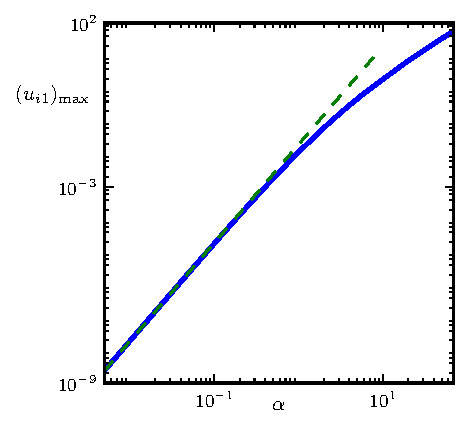
\includegraphics[width=0.5\textwidth]{Fig10}
        \label{fig:kn0.1:temp}
    }
    \subfloat[поле скоростей]{
        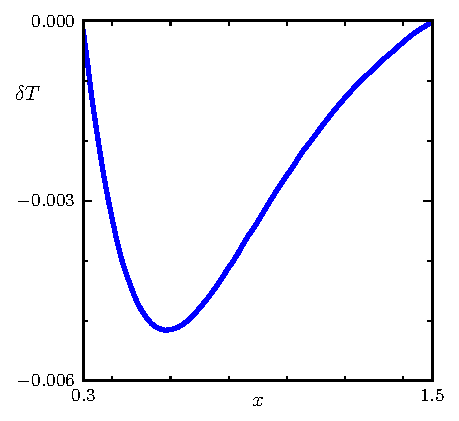
\includegraphics[width=0.5\textwidth]{Fig11}
        \label{fig:kn0.1:flow}
    }
    \caption{Решение уравнения Больцмана для \(\Kn=0.1\)}
    \label{fig:kn0.1}
\end{figure}

%%% Physical grid
Для рассмотрения задачи в произвольном диапазоне чисел Кнудсена необходимо
обратиться к численному решению уравнения Больцмана.
В физическом пространстве использовалась такая же разностная сетка,
как и при решении уравнений гидродинамического типа,
однако в слое Кнудсена (вблизи \(y=0\)) она дополнительно сгущалась так,
что ширина приграничной ячейки равнялась \(0.02\) от длины свободного пробега.

%%% Velocity grid
Для контроля точности в скоростном пространстве использовались несколько сеток (M1, M2, M3),
параметры которых представлены в табл.~\ref{table:velocity_grids}.
Сначала задача решалась на грубой равномерной прямоугольной сетке M1,
после чего результат уточнялся на неравномерных сетках.
В прямоугольной сетке M2 узлы вдоль осей \(x\) и \(z\) располагались как корни полинома Эрмита,
а вдоль оси \(y\) сгущались в геометрической прогрессии,
чтобы адекватно аппроксимировать сильный перепад функции распределения в слое Кнудсена.
В прямоугольной сетке M3 расстояние между узлами растёт квадратично вдоль каждой из осей.
В отличие от M2, холодные распределения (с температурой близкой к \(T=0.5\)) точнее аппроксимируются на M3.
Множества кубатурных точек также имели разную мощность: около \(5\cdot10^3\) для равномерной сетки
и около \(5\cdot10^4\) для неравномерной.
Кроме того, для очень малых \(\Kn\) применялась временн\'{а}я экстраполяция распределений
температуры и поля скоростей, поскольку достижение стационарного состояния вблизи \(y=1/2\)
требует слишком большого числа итераций явной схемы.

%%% Comparison of the velocity grids
При использовании неравномерных скоростных сеток необходимо учитывать не только качество аппроксимирования
функции распределения, но и точность кубатур вида~\eqref{eq:bzeta_cubature}.
Например, в последних двух столбцах табл.~\ref{table:velocity_grids} представлены диапазоны значений
невязки температуры максвеллиана \(\delta T_M\) и суммы двух полумаксвелианов \(\delta T_{MM}\)
для характерных температур и скоростей задачи.
На грубой сетке моменты функции распределения вычисляются достаточно точно,
если узлы распределены равномерно или как корни полинома Эрмита.
В противном случае необходимо использовать достаточно мелкую сетку,
как это сделано вдоль оси \(y\) для сетки M2.
Для сетки M3 кубатура~\eqref{eq:bzeta_cubature} для температуры всегда превышает истинное значение
на величину порядка \(0.004\), что позволяет скорректировать на эту величину поле температур,
получаемое из численного решения уравнения Больцмана.
Для сетки M1 невязка температуры принимает отрицательные значения для температур близких к \(T=1.5\),
поскольку используется недостаточное значение \(\zeta_{\mathrm{cut}}\).

%%% Results and discussions
На рис.~\ref{fig:kn0.01:temp} и~\ref{fig:kn0.01:flow} изображено поле температуры и скорости
для \(\Kn=0.01\) и проводится сравнение между численным решением уравнения Больцмана
и решением уравнений КГФ для малых \(\Kn\).
Отчётливо видно, что температурное поле, полученное с использованием
граничного условия старшего порядка (рис.~\ref{fig:kn0.01:temp-snit})
существенно лучше приближает точное решение (рис.~\ref{fig:kn0.01:temp-exact})
по сравнению с температурным полем, полученным без его использования (рис.~\ref{fig:continuum:temp-snit}).

На рис.~\ref{fig:kn0.1} показаны соответствующие распределения для \(\Kn=0.1\).
С увеличением \(\Kn\) возрастает поток теплового скольжения и температурный скачок возле границы \(y=0\).
При этом область максимальной скорости газа отодвигается от пластины.

\begin{figure}
    \scalebox{0}{
        
\begin{tikzpicture}
            \begin{axis}[hide axis]
                \addplot[line width=0.8, dotted](0,0);                      \label{leg:heat}
                \addplot[line width=0.8, dashed](0,0);                      \label{leg:asym0}
                \addplot[line width=0.8, dashdotted](0,0);                  \label{leg:asym1}
                \addplot[line width=0.8, solid](0,0);                       \label{leg:asym2}
                \addplot[line width=0.8, only marks, mark=o](0,0);          \label{leg:data1}
                \addplot[line width=0.8, only marks, mark=square](0,0);     \label{leg:data2}
                \addplot[line width=0.8, only marks, mark=triangle](0,0);   \label{leg:data3}
            \end{axis}
        \end{tikzpicture}
    }%
    \centering
    \subfloat[]{
        \includegraphics[width=0.5\textwidth]{Fig12}
        \label{fig:comparison:bottomT}
    }
    \subfloat[]{
        \includegraphics[width=0.5\textwidth]{Fig13}
        \label{fig:comparison:bottomU}
    }\\
    \subfloat[]{
        \includegraphics[width=0.5\textwidth]{Fig14}
        \label{fig:comparison:topT}
    }
    \subfloat[]{
        \includegraphics[width=0.5\textwidth]{Fig15}
        \label{fig:comparison:topU}
    }
    \caption{
        Некоторые граничные интегралы в зависимости от числа Кнудсена, полученные разными методами:
        уравнение теплопроводности~\ref{leg:heat},
        уравнения КГФ с тепловым скольжением~\ref{leg:asym0},
        с граничными условиями, содержащими только первые производные~\ref{leg:asym1},
        с граничными условиями, содержащими первые и вторые производные~\ref{leg:asym2},
        уравнение Больцмана на сетках M1~\ref{leg:data1}, M2~\ref{leg:data2} и M3~\ref{leg:data3}.
        Планка погрешности у M3 соответствует коррекции температурного поля в соответствии
        с невязкой температуры максвеллиана.
        Планка погрешности у M1 соответствует отностительной ошибке \(3\cdot10^{-4}\).
    }
    \label{fig:comparison}
\end{figure}

%%% Comparison between solutions
Чтобы наглядно продемонстрировать сходимость численного решения уравнения Больцмана к
решению уравнений КГФ в континуальном пределе, рассмотрим некоторые интегральные величины
в зависимости от числа Кнудсена (рис.~\ref{fig:comparison}).
На рис.~\ref{fig:comparison:bottomT} отчётливо видно, что граничные условия для гидродинамических уравнений
наряду с соответствующими коррекциями кнудсеновского слоя
аппроксимируют численное решение уравнения Больцмана с заявленной точностью.
В частности, условие~\eqref{eq:boundary_T0} даёт погрешность \(\OO{k}\),
учёт температурного скачка первого порядка приводит к \(\OO{k^2}\),
добавка линейного скачка второго порядка улучшает сходимость до \(\OO{k^3}\).
Отметим, что решение, полученное на грубой равномерной сетке M1, практически совпадает с решением на M2,
а также с откорректированным решением на M3.

На рис.~\ref{fig:comparison:bottomU} решение уравнения Больцмана соответствует погрешности \(\OO{k^2}\).
Посколько изображено поле \(v_i/k\), то погрешность существенно возрастает для малых \(k\).
Решения, полученные на неравномерных сетках, сгущающихся в области разрыва функции распределения (\(y=0\)),
совпадают между собой, но отличаются на константную величину (около \(0.008\)) от решения на M1.
Таким образом, разрыв функции распределения на границе диффузного отражения и затухание этого разрыва в слое Кнудсена
вносят незначительный вклад в общее решение задачи. Для медленных течений этот факт объясняется тем,
что величина разрыва равна \(\OO{k}\). Это наблюдение позволяет считать функцию распределения достаточно гладкой
без существенных потерь в точности, а, следовательно, можно пренебречь необходимостью адаптации скоростной сетки
к геометрии задачи.

На рис.~\ref{fig:comparison:topT} и~\ref{fig:comparison:topU}, как и ожидалось, гидродинамическое решение
отличается от кинетического на \(\OO{k}\), поскольку изображены интегральные величины,
вычисляемые вдали от границы диффузного отражения.
На рис.~\ref{fig:comparison:topT} отчётливо видно, что решение уравнения Больцмана сходится
именно к решению уравнений КГФ, а не уравнения теплопроводности,
при этом скорректированное решение на M3 практически совпадает с M2, немного превышая M1 (около 0.001).
Эта разница, по-видимому, объясняется грубой аппроксимацией сетки M1.
Кроме того, на рис.~\ref{fig:comparison:topT} и~\ref{fig:comparison:topU} видно,
что граничные условия, учитывающие вторые производные, слабо влияют на решение уравнений КГФ,
однако учёт только лишь температурного и скоростного скачков позволяет значительно улучшить точность
асимптотического решения для малых \(k\).

%%%%%%%%%%%%%%%%%%%%%%%%%%%%%%%%%%%%%%%%%%%
\subsection{Течение между двумя равномерно нагретыми эллиптическими цилиндрами}
%%%%%%%%%%%%%%%%%%%%%%%%%%%%%%%%%%%%%%%%%%%

\begin{figure}
    \centering
    \subfloat[уравнения КГФ с граничными условиями ведущего порядка]{
        \includegraphics{Fig16}
        \label{fig:elliptic:flow-kgf}
    }\\
    \subfloat[уравнения КГФ с граничными условиями, содержащими первые и вторые производные
    скорости и температуры]{
        \includegraphics{Fig17}
        \label{fig:elliptic:flow-asym}
    }
    \caption{Стационарное поле скоростей для \(\Kn=0.02\):
        изолинии соответствуют модулю, кривые со стрелками изображают направление}
\end{figure}

% allow break
\begin{figure}
    \ContinuedFloat % continue from previous page
    \subfloat[уравнение Больцмана]{
        \includegraphics{Fig18}
        \label{fig:elliptic:flow-kes}
    }
    \caption{(продолжение) Стационарное поле скоростей для \(\Kn=0.02\):
        изолинии соответствуют модулю, кривые со стрелками изображают направление}
    \label{fig:elliptic:flow}
\end{figure}

\begin{figure}
    \setcounter{subfigure}{0}
    \scalebox{0}{
        \begin{tikzpicture}
            \begin{axis}[hide axis]
                \addplot[line width=0.8, solid](0,0);       \label{leg:kes}
                \addplot[line width=0.8, dotted](0,0);      \label{leg:kgf}
                \addplot[line width=0.8, dashed](0,0);      \label{leg:first}
                \addplot[line width=0.8, dashdotted](0,0);  \label{leg:second}
            \end{axis}
        \end{tikzpicture}
    }%
    \centering
    \subfloat[внешний эллипс]{
        \includegraphics[width=0.5\textwidth]{Fig19}
        \label{fig:profile-temp:outer}
    }
    \subfloat[внутренний эллипс]{
        \includegraphics[width=0.5\textwidth]{Fig20}
        \label{fig:profile-temp:inner}
    }\\
    \subfloat[большая полуось внешнего эллипса]{
        \includegraphics[width=0.5\textwidth]{Fig21}
        \label{fig:profile-temp:bottom}
    }
    \subfloat[малая полуось внешнего эллипса]{
        \includegraphics[width=0.5\textwidth]{Fig22}
        \label{fig:profile-temp:left}
    }
    \caption{
        Профиль граничной температуры. Угол \(\varphi\) соответствует полярным координатам
        \(x=r\cos\varphi\), \(y=r\sin\varphi\). \(T_{\mathrm{HCE}}\) "--- поле температуры,
        описываемое уравнением теплопроводности.
        Представлены следующие решения: уравнение Больцмана~\ref{leg:kes} (поделённое на \(1.0017\)),
        уравнения КГФ с тепловым скольжением~\ref{leg:kgf},
        с граничными условиями, содержащими только первые производные~\ref{leg:first},
        с граничными условиями, содержащими первые и вторые производные~\ref{leg:second}.
    }
    \label{fig:profile-temp}
\end{figure}

\begin{figure}
    \centering
    \subfloat[внешний эллипс]{
        \includegraphics[width=0.5\textwidth]{Fig23}
        \label{fig:profile-vel:outer}
    }
    \subfloat[внутренний эллипс]{
        \includegraphics[width=0.5\textwidth]{Fig24}
        \label{fig:profile-vel:inner}
    }\\
    \subfloat[большая полуось внешнего эллипса]{
        \includegraphics[width=0.5\textwidth]{Fig25}
        \label{fig:profile-vel:bottom}
    }
    \subfloat[малая полуось внешнего эллипса]{
        \includegraphics[width=0.5\textwidth]{Fig26}
        \label{fig:profile-vel:left}
    }
    \caption{
        Профиль тангенциальной скорости границе. Угол \(\varphi\) соответствует полярным координатам
        \(x=r\cos\varphi\), \(y=r\sin\varphi\). Единичный вектор \(t_i\) направлен против часовой стрелки.
        Представлены следующие решения: уравнение Больцмана~\ref{leg:kes},
        уравнения КГФ с тепловым скольжением~\ref{leg:kgf},
        с граничными условиями, содержащими только первые производные~\ref{leg:first},
        с граничными условиями, содержащими первые и вторые производные~\ref{leg:second}.
    }
    \label{fig:profile-vel}
\end{figure}

%%% Formulation of the problem
Рассмотрим газ между двумя равномерно нагретыми коаксиальными эллиптическими цилиндрами,
расположенными так, что большие оси повёрнуты на угол \(\beta=\pi/2\).
\(a_0\) и \(b_0\) "--- полуоси внутреннего цилиндра, \(T_0\) "--- его температура,
\(a_1\) и \(b_1\) "--- полуоси внешнего цилиндра, \(T_1\) "--- его температура.
Численный анализ стационарной задачи для параметров
\[ a_0 = 0.3, \quad b_0 = 0.7, \quad T_0 = 1, \quad a_1 = 1.5, \quad b_1 = 1, \quad T_1 = 5 \]
представлен в литературе.
В частности, проведено статистическое моделирование (DSMC) для диапазона чисел
Кнудсена \(0.1\le\Kn\le5\) в~\cite{Sone1998}, исследована зависимость момента действующих
на цилиндры сил в зависимости от угла поворота \(\beta\) на основе уравнений КГФ в~\cite{Rogozin2014}.

%%% Aim of the study
В настоящей работе сравнивается численное решение уравнения Больцмана для молекулярной модели твёрдых сфер
и асимптотическое решение на основе уравнений КГФ с различными граничными условиями.
В силу симметрии задачи рассматривается первый квадрант (\(x>0\), \(y>0\)),
ось цилиндров находится в центре координат.
При различных числах Кнудсена возникают несколько видов течений.
В континуальном пределе поле скоростей во всей области имеет завихрённость против часовой стрелки~\cite{Sone2007,Rogozin2014},
обусловленную нелинейной термострессовой конвекцией,
но при \(\Kn>0.1\), наоборот, формируется течение по часовой стрелке,
которое доминирует над вихрем против часовой стрелки, находящимся в области,
наиболее удалённой от внутреннего цилиндра~\cite{Sone1998}.
Пристеночное течение по часовой стрелке образуется под действием тангенциального градиента температуры газа
на границе с диффузным отражением от равномерно нагретых цилиндров.
Процесс смены режима течения по мере роста \(\Kn\) до настоящего времени не был изучен численно,
картины конкурирующих течений также не представлены в литературе.
В частности, достижение приемлимого отношения сигнала к шуму при статистическом моделировании
нелинейной термострессовой конвекции требует колоссальных вычислительных затрат.

%%% Space discretization
Для численного решения задачи при \(\Kn=0.02\) в физическом пространстве
используется структурированная сетка, состоящая из \(N_V=2401\) четырёхугольных ячеек.
Она получается методом трансфинитной интерполяции с помощью пакета GMSH~\cite{gmsh2009}.
Направления продольных рёбер ячеек близки к касательным к изотермическим поверхностям,
а поперечных к градиенту температуры.
Вблизи цилиндрических поверхностей и особенно в области высокого градиента температур
сетка сгущается так, что минимальная ширина ячейки равна 0.046 длины свободного пробега.
В скоростном пространстве используется симметричная неравномерная сетка M4 (табл.~\ref{table:velocity_grids}),
в которой расстояние между узлами растёт квадратично вдоль каждой из осей.
Такая сетка позволяет удовлетворительно аппроксимировать функцию распределения
для широкого диапазона температур от \(T_0\) до \(T_1\).

%%% Information about consumed CPU time
Для нахождения стационарного решения уравнения Больцмана потребовалось \(10^5\) итераций,
при этом на каждом шаге использовалось \(5\cdot10^4\) кубатурных точек.
На персональном компьютере с CPU \(4\times3\)~GHz такой расчёт занял несколько суток.
На последних итерациях поля макроскопических величин усреднялись,
чтобы уменьшить шум, возникающий от циклического сдвига решётчатого правила Коробова
на случайный вектор.

%%% Results and discussions
На рис.~\ref{fig:elliptic:flow} изображены поля скорости, полученные различными методами.
Использование граничных условий для \(u_{iH2}\) (рис.~\ref{fig:elliptic:flow-asym}),
практически не меняет качественную картину течения по сравнению с классическими
граничными условиями для \(T_{H0}\) и \(u_{iH1}\) (рис.~\ref{fig:elliptic:flow-kgf}).
Следует отметить только общее понижение модуля скорости из-за скачка скорости,
а также термострессового скольжение второго порядка вдоль эллиптических поверхностей.
Численное решение уравнения Больцмана, однако, демонстрирует существенно отличную картину течения,
где наряду с термострессовой конвекцией против часовой стрелки возникает конкурирующий поток
в противоположном направлении. Этот поток наблюдается вне кнудсеновского слоя, но в области,
где градиент температуры и кривизна граничной поверхности максимальны,
поэтому он не может быть описан с помощью граничных условий.
Действительно, \(t_i\Pder[T_{H0}]{x_i}=0\) (\(t_i\) "--- единичный вектор касательный к границе),
поэтому на границе \(u_{iH1}=0\).
Термострессовое скольжение второго порядка сонаправлено с нелинейным термострессовым течением (\(a_4>0\)),
однако в следующем порядке члены, связанные с кривизной, пропорциональные \(\kappa t_i\Pder[T_{H1}]{x_i}\)
(\(\kappa\) "--- кривизна поверхности), уравновешивают пристеночное течение (\(\kappa(a_6+a_5/2)>0\)),
т.\,е. \(u_{iH2}t_i\) и \(u_{iH3}t_i\) имеют противоположный знак.
Численный анализ с нелинейными граничными условиями не проводился,
поскольку коэффициент перед членом \((t_i\Pder[T_{H1}]{x_i})(n_j\Pder[T_{H0}]{x_j})\) неизвестен.

%%% Remark on strong variation of the solution
Как видно из рис.~\ref{fig:elliptic:flow}, асимптотическое решение ведущего порядка некорректно описывает
поле скоростей уже при \(\Kn=0.02\). Действительно, геометрия задачи приводит к образованию области,
где нормальный градиент температуры оказывается сравним не с единицей, а с обратным числом Кнудсена,
что означает \(kn_i\Pder[f]{x_i} = \OO{f}\), причём в отличие от слоя Кнудсена градиент спадает медленно.
В такой области, строго говоря, асимптотическое решение в виде суммы~\eqref{eq:sum_solutions}
не может быть найдено, однако приближённая картина течения может быть уточнена
с помощью неизвестных до сих пор уравнений для \(T_{H1}\), \(u_{iH2}\) и \(p_{H3}\).
В этом случае асимптотическое решение следующего порядка является не поправкой порядка \(k\)
к основному, но сравнимым с ним.

%%% Extrapolation of the kesolver temperature field
Перед тем как сравнивать поля температур, уточним способ вычисления температуры
непосредственно на поверхностях цилиндров.
Дело в том, что численное решение уравнения Больцмана методом конечных объёмов
предоставляет значения функции распределения и макроскопических величин в центрах ячеек.
Поскольку в слое Кнудсена температура имеет слабую логарифмическую особенность,
то граничная температура вычисляется с помощью экстраполяции вида \(Ay\ln{y}+B\),
где \(A\) и \(B\) "--- константы, а \(y\) "--- расстояние от границы.
В предыдущей задаче линейной экстраполяции было достаточно,
поскольку ширина приграничной ячейки и градиент температуры были меньше.

%%% Comparison between solutions
Перейдём к рассмотрению рис.~\ref{fig:profile-temp} и~\ref{fig:profile-vel},
где показаны профили температуры и скорости на граничных поверхностях.
Использование температурного скачка первого порядка в граничных условиях
позволяет существенно улучшить асимптотическое поле температур,
в то время как температурный скачок следующего порядка является лишь малой поправкой.
Это связано с тем, что \(n_i\Pder[T_{H0}]{x_i}\) и \(n_in_j\Pderder[T_{H0}]{x_i}{x_j}\)
"--- величины одного порядка.
На рис.~\ref{fig:profile-temp} константное превышение численного решения над асимптотическим
в пределах \(0.004\) объясняется погрешностью кубатуры температуры,
однако на рис.~\ref{fig:profile-temp:left} и в области \(\varphi>\pi/3\) на рис.~\ref{fig:profile-temp:inner}
разница между решениями увеличивается из-за значительной разницы между скоростными полями \(u_i/k\),
влияющими на температурные поля через уравнение энергии~\eqref{eq:asymptotic1_T}.
Действительно, на рис.~\ref{fig:profile-vel:left} видно, что значение \((u_i/kT)\Pder[T]{x_i}\)
отличается даже знаком.
Граничные условия, содержащие вторые производные, позволяют лучше приблизить численное решение
на внешнем цилиндре (рис.~\ref{fig:profile-vel:outer}), но не на внутреннем (рис.~\ref{fig:profile-vel:inner}).
Как было указано выше, это связано с тем, что в области максимального градиента температуры
граничные условия для \(u_{iH3}\) в общем случае имеют порядок \(\OO{u_{iH2}/k}\),
но они не учтены при решении уравнений КГФ. Резкие колебания численного решения уравнения Больцмана
(особенно на рис.~\ref{fig:profile-vel:inner}) обусловлены погрешностью дискретизации в скоростном пространстве,
но не превышают \(10^{-4}\) по абсолютному значению \(u_i\).

%%%%%%%%%%%%%%%%%%%%%%%%%%%%%%%%%%%%%%%%%%%
\section{Заключение}
%%%%%%%%%%%%%%%%%%%%%%%%%%%%%%%%%%%%%%%%%%%

%%% Projection method
На нескольких численных примерах был проведен анализ медленных неизотермических течений
слаборазреженного газа, а также их влияния на температурное поле.
С помощью проекционно-интерполяционного метода дискретных скоростей удалось получить картины течений
с точностью, практически недостижимой с помощью традиционного метода DSMC.
Основную сложность представляет проблема дискретизации скоростного пространства
для обеспечения удовлетворительной аппроксимации функции распределения в задачах с большим перепадом температур.
В настоящей работе эта проблема была решена с помощью неравномерных сеток в пространстве скоростей,
которые, однако, приводят к дополнительным вычислительным трудностям.
В частности, усложняется алгоритм консервативного проецирования в интеграле столкновений,
повышаются требования к мощности множества кубатурных точек,
что в целом приводит к увеличению вычислительных затрат.
Кроме того, на неравномерной сетке, в общем случае, уменьшается точность кубатур
функций близких к максвелловским, характерных для медленных течений.
Тем не менее, полученные численные решения с высокой точностью совпадают с
результатами асимптотического анализа уравнения Больцмана при малых числах Кнудсена.
Таким образом, проекционно-интерполяционный метод на неравномерных сетках
может быть рекомендован для моделирования широкого спектра медленных неизотермических течений
слаборазреженного газа.

%%% Range of applicability of the KGF equations
С помощью численного решения уравнения Больцмана для газа твёрдых сфер было показано,
что уравнения Когана"--~Галкина"--~Фридлендера с соответствующими граничными условиями
адекватно описывают медленные неизотермические течения газа при достаточно малых числах Кнудсена.
Если в задаче присутствует такая область, где на средней длине свободного пробега температура
газа изменяется на величину, сравнимую с её характерным значением, то уравнения гидродинамического типа
не применимы для описания разреженного газа в этой области. Корректное описание может предоставить
только кинетический подход.

%%% On boundary conditions
Было показано, что использование граничных условий, учитывающих, наряду с тепловым скольжением,
температурный и скоростной скачки первого порядка,
существенно улучшают точность асимптотического решения, так как для рассматриваемых задач
характерны большие значения градиента температуры вдоль нормали к граничной поверхности.
Учёт членов следующего порядка в граничных условиях к уравнениям КГФ даёт лишь малую поправку.

%%% About coefficients and Knudsen-layer functions
Коэффициенты в граничных условиях, вместе с функциями-корректорами кнудсеновского слоя,
получаются из численных решений соответствующих одномерных задач кнудсеновского слоя.
В настоящее время они известны лишь для модельного уравнения Крука"--~Веландера,
а также для простейшего потенциала твёрдых сфер, что существенно ограничивает применение
в прикладных задачах.
Более того, задача кнудсеновского слоя для нелинейных членов, которая сводится к неоднородному
линеаризованному уравнению Больцмана, не решена даже для потенциала твёрдых сфер.

\section*{Благодарности}

Автор признателен О.\,Г. Фридлендеру за плодотворные дискуссии,
послужившие отправной точкой к настоящему исследованию,
В.\,С. Галкину за подробные и ценные замечания, позволившие улучшить изложение материала,
а также Ф.\,Г. Черемисину за поддержку и внимание к работе.

\bibliographystyle{maik}
\bibliography{manuscript}

\end{document}


